\newcommand{\valorIliquidezM}{1}
\newcommand{\valorIliquidezm}{984}
\newcommand{\valorIliquidezc}{766}
\newcommand{\valorIliquidez}{\valorIliquidezM,\valorIliquidezm,\valorIliquidezc}
\newcommand{\valorIliquidezLetra}{\Numberstringnum{\valorIliquidezM}{} millones, \numberstringnum{\valorIliquidezm}{} mil, \numberstringnum{\valorIliquidezc}}


\subsection{ESTIMACI\'ON DEL DEM\'ERITO POR FALTA DE LIQUIDEZ DE UNA PARTICIPACIÓN ACCIONARIA PRIVADA Y MINORITARIA.}

El marco te\'orico de las finanzas de valuaci\'on establece que la venta de una participaci\'on accionaria privada presenta una dificultad importante para concretarse y realizarse en efectivo.

\begin{figure}[H]
\centering
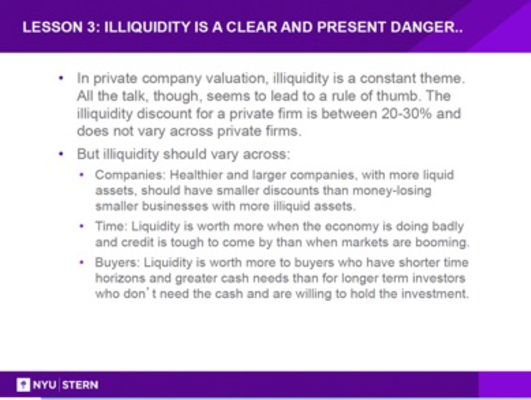
\includegraphics[width=8cm]{\rutaImagenes/liquidity_1}
\end{figure} 

Cuando un accionista determinado detenta un paquete accionario minoritario donde requiere compartir sus decisiones al ejercer sus derechos corporativos y econ\'omicos con otros accionistas ya establecidos; siempre resulta menos atractiva de venderse. A dicho descuento se le conoce como descuento por iliquidez (illiquidity discount):

\begin{figure}[H]
\centering

\includegraphics[width=8cm]{\rutaImagenes/liquidity_2}
\end{figure} 

Por lo anterior, el valuador llev\'o a cabo un estudio de diversas publicaciones (papers) de consultoras financieras, habi\'endose estimado un dem\'erito de \textcolor{principal}{\textbf{26.85\% (D. Rate \%)}}, lo cual corresponde a la media ponderada; buscando dar mayor importancia a los dem\'eritos m\'as peque\~nos de la muestra a juicio del valuador, seg\'un se aprecia:

\begin{figure}[H]
\centering
\includegraphics[width=16cm]{../0.imagenes/tasa_demerito_1}
\end{figure} 

Una vez estimado dicho dem\'erito, se aplica la f\'ormula del factor de dem\'erito por liquidez, obteni\'endose el cociente: 

\begin{figure}[H]
\centering
Factor de descuento por iliquidez $= 1 – D. Rate$ \%\\

\includegraphics[width=12cm]{../0.imagenes/tasa_demerito_2}
\end{figure} 

A continuaci\'on se concluye el valor razonable ajustado del capital accionario (\textit{Equity Adjusted Value}), a la fecha de valores:

\begin{table}[H]
\centering
\begin{tabular}{p{10cm}m{3cm}}
\begin{minipage}{10cm}
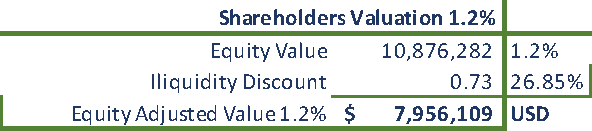
\includegraphics[width=10cm]{../0.imagenes/tasa_demerito_3}\\


\end{minipage}&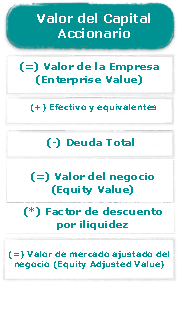
\includegraphics[width=3cm]{\rutaImagenes/valor_capital_accionario}
\end{tabular}
\\
Valor razonable de la participación accionaria minoritaria del 29.71\%: \textcolor{principal}{\textbf{\$\valorIliquidez MXN.}}
\end{table}

%\begin{figure}[H]
%\centering
%Tipo de cambio al 31/12/2021: \textcolor{principal}{\textbf{20.5157}}\\[10pt]
%
%
%\includegraphics[width=12cm]{../0.imagenes/tasa_demerito_4}\\[10pt]
%
%Valor razonable de la participaci\'on accionaria minoritaria\\
%del 1.2\% en Pesos Mexicanos (Cifras redondeadas): \\[10pt]
%
%\textcolor{principal}{\textbf{\$163'225,150.00 MXN}}\\[10pt]
%
%\textcolor{principal}{\textbf{(Ciento sesenta y tres millones, doscientos veinticinco mil,}} \\
%\textcolor{principal}{\textbf{ciento cincuenta pesos 00/100 Moneda Nacional)}}
%
%
%
%
%
%
%
%\end{figure}

